\documentclass[a4paper, 10pt]{article}
\usepackage[top=2.0cm,bottom=2.0cm,left=1.5cm,right=2.5cm]{geometry}

\usepackage{float}
\usepackage{hyperref}
\hypersetup{
  colorlinks   = true,   % Colours links instead of ugly boxes
  urlcolor     = red,    % Colour for external hyperlinks
  linkcolor    = red,    % Colour of internal links
  citecolor    = red     % Colour of citations
}

\usepackage[ngerman]{babel}
\usepackage[ansinew]{inputenc}

% Notes am rechten Seitenrand -deshalb die unterschiedliche Breite.
\usepackage{marginnote}

\usepackage{amssymb}
\usepackage{amsmath}
\usepackage{amstext}
\usepackage{amsfonts}
\usepackage{eurosym}
\usepackage{trfsigns}

\usepackage{longtable}
\usepackage{tabularx}
\usepackage{multirow}
\usepackage[table]{xcolor}
\usepackage{graphicx}
\usepackage{booktabs}% http://ctan.org/pkg/booktabs
\newcommand{\tabitem}{~~\llap{\textbullet}~~}

\usepackage{tcolorbox}
\usepackage{pdflscape}

\tcbuselibrary{breakable,skins}
\usepackage{ctable}
\definecolor{darkgreen}{RGB}{0,136,0 }
\definecolor{violett}{RGB}{154,50,205 }
\definecolor{htwgreen}{RGB}{134,189,36 }

% alternate rowcolors for all long-tables
\let\oldlongtable\longtable
\let\endoldlongtable\endlongtable
\renewenvironment{longtable}{\rowcolors{2}{white}{lightgray}\oldlongtable} {
\endoldlongtable}

% Definition
% #1: Title
% #2: Bemerkung
\newcounter{def}
\newtcolorbox{defbox}[3][]{
  enhanced,
  overlay unbroken and first={ 
\node[fill=white,rounded corners, draw=white, text=gray, line width=3pt, inner sep=4pt, anchor=east, xshift=-10pt] at (frame.north east){#2};
\node[anchor=north east, text=gray, fill=white, text width=3.5em, align=left, minimum height=4ex] at ([xshift=4.5\marginparsep]frame.north east) {\small Def. \stepcounter{def}\thedef \newline \textcolor{black}{#3} };
}, 
  colframe=gray, 
  %colback=mytestcolor, 
  colback=white, 
  coltitle=red!70!gray, 
  boxrule=1pt, 
  arc=1mm, 
  breakable,
  top=5pt,
  before=\vskip18pt}

% Satz
% #1: Title
% #2: Bemerkung
\newcounter{satz}
   \newtcolorbox{theorembox}[3][]{
  enhanced,
  overlay unbroken and first={ 
\node[fill=white,rounded corners, draw=white, text=gray, line width=3pt, inner sep=4pt, anchor=east, xshift=-10pt] at (frame.north east){#2};
\node[anchor=north east, text=gray, fill=white, text width=3.5em, align=right, minimum height=4ex] at ([xshift=4.5\marginparsep]frame.north east) {\small Regel \stepcounter{satz}\thesatz \newline \textcolor{black}{#3} };
}, 
  colframe=gray, 
  %colback=mytestcolor, 
  colback=white, 
  coltitle=red!70!gray, 
  boxrule=1pt, 
  arc=1mm, 
  breakable,
  top=5pt,
  before=\vskip18pt
}

% Beispiel
% #1: Title
% #2: Bemerkung
\newcounter{exa}
\newtcolorbox{exabox}[3][]{
  enhanced,
  overlay unbroken and first={ 
	  \node[fill=white, rounded corners, draw=white, text=blue, line width=3pt, inner sep=4pt, anchor=east, xshift=-10pt] at (frame.north east) {#2}; 
	  \node[anchor=north east, text=blue, fill=white, text width=3.5em, align=right, minimum height=4ex] at ([xshift=4.5\marginparsep]frame.north east)  {\small  Bsp \stepcounter{exa}\theexa \newline \textcolor{black}{ #3} };
}, 
  colframe=blue, 
  colback=white, 
  coltitle=red!70!blue, 
  boxrule=1pt, 
  arc=1mm, 
  breakable,
  top=5pt,
  before=\vskip18pt
}

% �bung
% #1: Title
% #2: Bemerkung
\newcounter{exercise}
\newtcolorbox{exercisebox}[1][]{
  enhanced,
  overlay unbroken and first={ 
	  \node[fill=white, rounded corners, draw=white, text=black, line width=3pt, inner sep=4pt, anchor=east, xshift=-10pt] at (frame.north east)  {#1}; 
	  \node[anchor=north east, text=black, fill=white, text width=3.5em, align=right, minimum height=4ex] at ([xshift=4.5\marginparsep]frame.north east)  
	  {\small  Aufg. \stepcounter{exercise}\theexercise };
}, 
  colframe=black, 
  colback=white, 
  coltitle=red!70!blue, 
  boxrule=1pt, 
  arc=1mm, 
  breakable,
  top=5pt,
  before=\vskip18pt
}

\usepackage{fancyhdr}
\pagestyle{fancy}
\fancyfoot[C]{\footnotesize
    Prof. Dr. Lucy Weggler -- Lizenz:
    \href{https://creativecommons.org/licenses/by-nc-sa/4.0/}{CC-BY-NC-SA 4.0}
    \hfill \thepage
}

% Gemeinsame Kopfzeile: eine Hauptueberschrift, links, klein und aufrecht.
% Die Fusszeilen werden weiterhin im jeweiligen Hauptdokument festgelegt.
\makeatletter
\@ifpackageloaded{scrlayer-scrpage}{%
  % Im gegliederten Gesamtskript ist das Kapitel die Hauptueberschrift.
  \automark{chapter}
  \setkomafont{pagehead}{\normalfont\footnotesize}
  \ihead{}\chead{}\ohead{}
  \lehead{\headmark}
  \lohead{\headmark}
}{%
  % In den article-Dokumenten ist section die oberste Gliederungsebene.
  \fancyhead{}
  \fancyhead[L]{\normalfont\footnotesize\nouppercase{\leftmark}}
  \renewcommand{\sectionmark}[1]{\markboth{\thesection\quad #1}{}}
  \renewcommand{\subsectionmark}[1]{}
  \setlength{\headheight}{14pt}
}
\makeatother


% Aufgaben gemeinsam mit der Theorie verlinken; siehe LaTeX/README.md.
% Einmal in der Praeambel des Hauptdokuments nach hyperref laden.
% true: Theorie, Aufgaben und Loesungen gemeinsam; false: getrennte Ausgaben.
\newif\ifintegriereaufgaben
\integriereaufgabenfalse

% Fuehrt den gesamten Inhalt nur bei vorhandenem Label aus.
% Wie normale Querverweise benoetigt die Erkennung mehrere LaTeX-Laeufe.
\newcommand{\wennreferenzvorhanden}[2]{%
  \ifcsname r@#1\endcsname
    #2%
  \fi
}

% Verlinkte Nummer bei vorhandenem Ziel, andernfalls keinerlei Ausgabe.
\newcommand{\abschnittsverweis}[1]{%
  \wennreferenzvorhanden{#1}{\ref{#1}}%
}

% Gleichbedeutender Name fuer bestehende Theoriehinweise.
\newcommand{\skriptverweis}[1]{\abschnittsverweis{#1}}

% Ohne Ziel wird auch kein leerer Randnotiz-Kasten angelegt.
\newcommand{\randverweis}[1]{%
  \wennreferenzvorhanden{#1}{\marginpar{\small\abschnittsverweis{#1}}}%
}

\integriereaufgabenfalse

\begin{document}
\pagenumbering{roman}

\section*{\LARGE Mathematische Grundlagen}

\section*{Leitidee}

Mathematik ben�tigt eine pr�zise Sprache, um Objekte, Aussagen und
Zusammenh�nge eindeutig zu beschreiben. \textbf{Mengen und Logik} bilden
daf�r das formale Fundament.

Die \textbf{Zahlenmengen} legen fest, welche Objekte f�r mathematische
Operationen zur Verf�gung stehen und nach welchen algebraischen Regeln
mit ihnen gerechnet werden kann. Auf dieser Grundlage erm�glichen
\textbf{�quivalenzumformungen}, Gleichungen und Ungleichungen systematisch
zu untersuchen und L�sungs- oder Definitionsmengen zu bestimmen.

 

\bigskip

\tableofcontents
\newpage

\pagenumbering{arabic}
\setcounter{section}{0}
% Mengen und Logik
\setcounter{satz}{0} \setcounter{def}{0} \setcounter{exa}{0}  
\section{Mengen und Logik}\label{MA1-mengen-und-logik}

\begin{table}[H]
  \centering
  \begin{tabularx}{\textwidth}{p{0.9\textwidth} p{0.1\textwidth}}
    \toprule
	  \multicolumn{2}{c}{\textbf{�bersicht �ber Lernziele und Voraussetzungen}}\\
    \midrule
	  \textbf{Lernziele} &\\[.5\normalbaselineskip]
    \tabitem Mengen in mathematischer Symbolsprache korrekt formulieren &\\
    \tabitem mathematische Aussagen pr�zise aufschreiben &\\ 
    \tabitem mathematische Formelsprache lesen und interpretieren &\\
    \bottomrule
  \end{tabularx}
\end{table}

\ifintegriereaufgaben \noindent �bungsaufgaben zum Thema sind hier: \hyperref[MA1-mengen-und-logik-aufgaben]{Aufgaben}
\vspace{0.3cm}
\hrule
\fi

\subsection{Was ist eine Menge in der Mathematik?}

Mit Hilfe von Mengen kann man fast alle mathematischen Objekte beschreiben. Ob die Zahl $7$, ein Kreis in der Ebene, die Relation "$\leq$"\, oder die Sinus-Funktion: all diese Objekte kann man als mehr oder weniger komplizierte Menge angeben! In der Mathematik wird eine Menge durch geschwungene Klammern angezeigt: \( \{ \}\). Zwischen den Klammern notiert man die Elemente der Menge. Eine Menge (\emph{set}) kann man sich vorstellen wie einen Beutel, in dem Elemente drin stecken und f�r die Elemente gelten folgende Eigenschaften:  
\begin{theorembox}{Eigenschaften einer Menge}{}
  \begin{itemize}
	  \item Die Reihenfolge der Elemente einer Menge ist egal. F�r eine Menge $M$, deren Elemente die drei Zahlen  \(1, 2 \) und \(3\) sind, gilt also: 
      $$ M = \{ 1, 2, 3\} = \{ 2, 1, 3\} = \{ 3, 1, 2\}= \{ 1, 3, 2\}= \{ 2, 3, 1\}= \{ 3, 2, 1\}\,. $$
    \item Wird ein Element in einer Menge mehrfach notiert, �ndert dies die Menge nicht. Beispielsweise gilt 
	    $$ M = \{ 1, 2, 2, 3\} = \{ 1, 2, 3\}\,. $$ 
	    Entscheidend ist also nur, \textbf{ob} ein Elmeent zur Menge geh�rt, nicht wie oft es bei der Beschreibung aufgef�hrt wird.
  \end{itemize}
  \end{theorembox}
  
  \noindent{\textbf{Bemerkungen:}}

\begin{itemize} 
	\item Mengen verhalten sich also anders als Zahlenpaare (Tupel wie \((1,2)\) oder Tripel \( (1,2,3)\)), die man von Koordinaten kennt - da spielt n�mlich die Reihenfolge eine wesentliche Rolle. 
	\item Um auszuschlie�en, dass Elemente einer Menge doppelt vorkommen, m�sste man immer explizit sagen, dass die Elemente unterschiedlich sind. Oft wird das implizit vorausgesetzt. Auf jeden Fall sollte man aufpassen, gilt zum Beispiel $x=y=z$, dann enth�lt die Menge $\{x,y,z\}$ nur ein Element und nicht drei. 
\end{itemize}

F�r  "$x$ ist Element von $M$"\, bzw. "$x$ ist nicht Element von $M$"\, schreibt man: 

\begin{defbox}{(kein) Element einer Menge}{}
  $x \in M \textnormal{ bzw. } x \not \in M\,.$
\end{defbox}

Es gibt nur eine Menge ohne Elemente: die leere Menge. Sie wird auf zwei Weisen geschrieben:

\begin{defbox}{Leere Menge}{ }
  $\emptyset$ oder $\{ \}\,.$
\end{defbox}

F�r die M�chtigkeit, also die Anzahl der Elemente einer Menge $M$, schreibt man \(|M|\), also:

\begin{exabox}{M\"achtigkeit}{ }
	$ \big|\emptyset \big| = 0, \quad \big|\{ -2,\frac32, 0, *\}\big| = 4 \,.$
\end{exabox}

Im  Falle  einer unendlichen Menge, also  einer  Menge  mit  unendlich  vielen Elementen, ergibt das keine endliche Zahl, sondern "\,unendlich"\footnote{Es gibt verschiedene Arten von Unendlich, wie Georg Cantor schon $1877$ herausgefunden hat.}. In dem Fall schreiben wir  $|M| = \infty$.

\subsubsection*{Verkn�pfungen von Mengen}

Wenn jedes Element einer Menge $A$ auch Element einer Menge $B$ ist, dann ist $A$ eine Teilmenge von $B$ und $B$ eine Obermenge von $A$. Man schreibt $A\subset B$. Am schnellsten l�sst sich das erfassen mit einer Skizze: 
  
\begin{exabox}{Teilmenge und Obermenge}{ }
\begin{minipage}{0.3\textwidth}
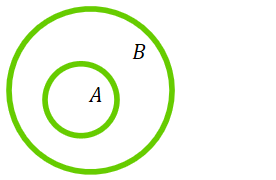
\includegraphics{../Mathematik_1/Bilder/mengen_echte_teilmenge.png} %Diagramm / Beispiel
\end{minipage}
\begin{minipage}{0.7\textwidth}
	\begin{itemize} 
	\item \(A\) ist eine Teilmenge von \(B\): \(A\subseteq B\)
	\item \(B\) ist eine Obermenge von \(A\): \(A\subseteq B\)
	\item \(A\) ist nicht gleich \(B\): \(A\not = B\)
	\item \(A\) ist eine \textbf{echte} Teilmenge von \(B\): \(A\subsetneq B\)
\end{itemize}
\end{minipage}
\end{exabox}
  
Zwei Mengen \(A\) und \(B\) sind gleich, \(A=B\), wenn sie dieselben Elemente enthalten. 

In der Mengenlehre gibt es vier grundlegende Mengenoperationen, n�mlich: Vereinigung, Schnitt, Differenz und Komplement: 

\begin{exabox}{Mengenoperationen}{}
	\begin{itemize}
		\item Die Vereinigung  (\emph{union}) zweier Mengen wird mit dem Symbol \(\cup\) angezeigt. Die Vereinigungsmenge enth�lt jedes Element der beiden Mengen genau einmal, beispielsweise
	\[ \{ 1, 2, 4\} \cup \{2, 5, 3, 4\} = \{1,2,3,4,5\}\,. \]
\item Der Schnitt (\emph{intersection}) zweier Mengen wird mit dem Symbol \(\cap\) angezeigt. Die Schnittmenge enth�lt jedes Element, das in beiden Mengen vorkommt, beispielsweise 
	\[ \{ 1, 2, 4\} \cap \{2, 5, 3, 4\} = \{2,4\}\,. \]
\item Die Differenz (\emph{difference}) zweier Mengen wird mit einem Backslash angezeigt. Die Differenzmenge enth�lt jedes Element, das in der ersten Menge vorkommt, aber nicht in der zweiten, beispielsweise 
	\[ \{ 1, 2, 4\} \setminus \{2, 5, 3, 4\} = \{1\}\,.\]
\item Das Komplement (\emph{complement}) einer Menge \(A\) wird mit einem waagerechten Strich �ber der Menge angezeigt, also \(\overline A\). Ist eine Obermenge \(B\) von \(A\) fixiert, dann bedeutet das Komplement \(\overline A\) die Differenz von Obermenge \(B\) und \(A\). Aus der Schreibweise \(\overline A\) geht die Obermenge nicht hervor - die Obermenge muss also implizit bekannt sein! Im folgenden Beispiel ist die Obermenge die Menge der nat�rlichen Zahlen ohne die Null, also $\mathbb N = \{ 1, 2, 3, 4, 5, 6, \dots\}$: 
	\[ \overline{\{2, 4, 6, 8\}} = \mathbb N \setminus \{2, 4, 6, 8\} = \{1,3,5,7\} \cup \{9,10,11,12, \dots\}\,. \]
	\end{itemize}
\end{exabox}

Neben den bisher betrachteten Mengenoperationen gibt es eine weitere wichtige M�glichkeit, aus gegebenen Mengen eine neue Menge zu bilden. Dabei werden die Elemente der beiden Mengen nicht vereinigt oder miteinander verglichen, sondern zu \textbf{geordneten Paaren} zusammengesetzt.

F�r zwei Mengen \(A\) und \(B\) hei�t

$$
A\times B
=
\{(a,b):a\in A \text{ und } b\in B\}
$$

das kartesische Produkt (\emph{cartesian product}) von \(A\) und \(B\).

Anders als bei den Elementen einer Menge spielt innerhalb eines geordneten Paares die Reihenfolge eine Rolle. Im Allgemeinen gilt daher

$$
(a,b)\neq(b,a).
$$

Das passt zu dem bereits bekannten Unterschied zwischen Mengen und Tupeln: W�hrend beispielsweise

$$
\{2,3\}=\{3,2\}
$$

gilt, sind die geordneten Paare

$$
(2,3)\neq(3,2)
$$

verschieden.

\begin{exabox}{Kartesisches Produkt}{ }
F�r

$$
A=\{\circ,\diamond,M\}
\qquad\text{und}\qquad
B=\{3,7\}
$$

ergibt sich

$$
\begin{aligned}
A\times B
=
\{&
(\circ,3),(\circ,7),
(\diamond,3),(\diamond,7),\\
&
(M,3),(M,7)
\}.
\end{aligned}
$$

Jedes Element aus \(A\) wird dabei mit jedem Element aus \(B\) kombiniert.
\end{exabox}

Besonders wichtig ist das kartesische Produkt einer Menge mit sich selbst. F�r die reellen Zahlen gilt beispielsweise

$$
\mathbb R^2
:=
\mathbb R\times\mathbb R
=
\{(x,y):x\in\mathbb R \text{ und } y\in\mathbb R\}.
$$

Die Elemente von \(\mathbb R^2\) sind also geordnete Paare reeller Zahlen. Sie k�nnen geometrisch als Punkte der Ebene interpretiert werden.

Entsprechend entstehen durch weitere kartesische Produkte geordnete Tripel und allgemein geordnete \(n\)-Tupel. Beispielsweise ist

$$
\mathbb R^3
=
\{(x,y,z):x,y,z\in\mathbb R\}
$$

die Menge aller geordneten Tripel reeller Zahlen und kann als Menge der Punkte des dreidimensionalen Raumes aufgefasst werden.
  
Entsprechend zu "\,Punktrechnung vor Strichrechnung"\, wird der Schnitt vor der Vereinigung ausgef�hrt:
\begin{theorembox}{Rechenregel: Schnitt vor Vereinigung}{ }
$  A \cup B \cap C = A \cup \left( B \cap C\right) \,.  $
\end{theorembox}

\subsection{Was ist eine mathematische Aussage?}

Eine  mathematische Aussage (\emph{statement,  proposition}) ist eine Aussage, der man einen Wahrheitswert zuordnen kann. Entweder ist die Aussage wahr (\emph{true}) oder falsch (\emph{false}). Eine mathematische Aussage kann aus diesem Grund \textbf{keine} freien Variablen enthalten. Wenn freie Variablen vorkommen, handelt es sich um ein Pr�dikat. Man nennt ein Pr�dikat auch "\,eine Aussageform"\, oder einfach "\,ein mathematischer Ausdruck"\,:
  
\begin{exabox}{Aussagen und Pr�dikate}{ }
  \begin{itemize}
  \item "$2^2 = 5$"\, ist eine falsche Aussage.
    \item "$2^2 \not= 5$" \; ist eine wahre Aussage.
    \item "$x^2 \in \mathbb N$" \; ist ein Pr�dikat.
  \end{itemize}
\end{exabox}

  
\begin{exabox}{Aussagen}{ }
  \begin{itemize}
	  \item "\,F�r eine beliebige nat�rliche Zahl $x\in \mathbb N$ gilt $x^2 \in \mathbb N$"\; ist eine wahre Aussage.
	  \item "\,F�r eine beliebige rationale Zahl $x\in \mathbb Q$ gilt  $x^2 \in \mathbb N$"\; ist eine falsche Aussage.
  \end{itemize}
\end{exabox}
Mathematische Aussagen treten selten isoliert auf. H�ufig m�chte man Aussagen \textbf{verneinen} oder mehrere Aussagen miteinander \textbf{verkn�pfen}. Auch daf�r besitzt die Mathematik eine eigene Kurzschreibweise.

Beginnen wir mit der Negation oder Verneinung. Betrachten wir die Aussage

$$
p:\qquad x\geq 0.
$$

Diese Aussage ist beispielsweise f�r \(x=3\) wahr und f�r \(x=-2\) falsch. M�chte man genau das Gegenteil von \(p\) ausdr�cken, so lautet die entsprechende Aussage:

$$
q: \qquad x<0.
$$

In Worten k�nnte man auch sagen: �Es gilt \textbf{nicht} \(x\geq0\).�

Die Aussage \(q\) ist die Negation (\textit{negation}) von \(p\) und das l�sst sich in mathematischer Formelsprache mit Hilfe des Symbols \(\neg\) ausdr�cken: die Negation von \(p\) ist 

$$
\neg p.
$$

Eine Negation \(\neg p\) ist genau dann wahr, wenn die urspr�ngliche Aussage \(p\) falsch ist -- und umgekehrt.

\begin{exabox}{Negation einer Aussage}{ }
	\begin{itemize}
\item F�r $ \; p:\qquad x\geq 0\; $ lautet die Negation $ \;\neg p:\qquad x<0$.
\item Beispielsweise ist f�r \(x=-2\) die Aussage \(p\) falsch und die Aussage \(\neg p\) wahr.
	\end{itemize}
\end{exabox}

Neben der Negation einer einzelnen Aussage m�chte man Aussagen auch miteinander verbinden. Betrachten wir beispielsweise die Aussage \( p:\; x>2\) und die Aussage \(q:\; x<5\). Suchen wir alle reellen Zahlen, f�r die \textbf{sowohl}  \(p\) \textbf{als auch} \(q\) gleichzeitig wahr ist, so verkn�pfen wir die Aussagen durch ein logisches �und�. In mathematischer Formelsprache ist das logische �und� das Symbol \(\land\):

$$
p\land q: \qquad x>2 \;\textnormal{und gleichzeitig} \; x<5.
$$
Eine Und-Verkn�pfung (\emph{and}) \(p\land q \) ist genau dann wahr, wenn sowohl \(p\) als auch \(q\) wahr sind.

Suchen wir alle reellen Zahlen, f�r die \textbf{mindestens eine der Aussagen}, wahr ist, so verkn�pfen wir die Aussagen durch ein logisches �oder� . In mathematischer Formelsprache ist das logische �oder�  das Symbol \(\lor\): 

$$
p\lor q: \qquad x>2 \;\textnormal{oder}\; x<5.
$$
Eine Oder-Verkn�pfung (\emph{or}) \(p\land q \) ist genau dann wahr, wenn  mindestens eine der beiden Aussagen \(p\) und \(q\) wahr ist.

\begin{exabox}{Und und Oder lesen}{ }
	Es seien $ p:\; x>2$ und $q:\; x<5 $.
	\begin{itemize}
		\item $ p\land q $ bedeutet in Worten  �\(x\) ist gr��er als \(2\) und gleichzeitig kleiner als \(5\).� und  diese Aussage ist  genau dann wahr wenn $ 2<x<5 $.  
		\item $ p\lor q $ bedeutet in Worten  �\(x\) ist gr��er als \(2\) oder kleiner als \(5\).� und diese Aussage ist genau dann wahr wenn \(x>2\) oder \(x<5\) wahr ist, wobei auch beide Bedingungen gleichzeitig erf�llt sein d�rfen (aber nicht m�ssen).
	\end{itemize}
\end{exabox}

\noindent{\textbf{Bemerkungen:}}
\begin{itemize}
	\item Die Symbole \(\neg\), \(\land\) und \(\lor\) werden uns immer wieder begegnen. Sie sind nicht nur Bestandteil der Aussagenlogik, sondern geh�ren zur mathematischen Formelsprache. 
	\item Bei der Beschreibung von Mengen werden wir Bedingungen mit diesen Operatoren sinnvoll verkn�pfen. Deshalb ist es wichtig, logische Ausdr�cke nicht nur selbst aufschreiben, sondern auch in nat�rliche Sprache �bersetzen zu k�nnen.
	\item Beim mathematischen Oder ist das Wort �oder� einschlie�lich zu verstehen: Sind \(p\) und \(q\) beide wahr, dann ist auch \(p\lor q\) wahr. Das unterscheidet das mathematische Oder von Formulierungen wie �entweder -- oder�, bei denen h�ufig gemeint ist, dass genau eine von zwei M�glichkeiten eintreten soll.
\end{itemize}

Entsprechend zu �Punktrechnung vor Strichrechnung� gibt es auch f�r logische Operatoren eine festgelegte Reihenfolge: Zuerst wird die Negation ausgef�hrt, danach das Und und zuletzt das Oder.

\begin{exabox}{Klammern weglassen?}{ }
Betrachten wir den vollst�ndig geklammerten Ausdruck

$$
\bigl(\neg(x\geq 6)\bigr)\lor\bigl((x\geq 10)\land(x<20)\bigr).
$$

Welche Klammern k�nnen weggelassen werden, ohne die Bedeutung des Ausdrucks zu ver�ndern?

Da die Negation \(\neg\) vor dem Und \(\land\) und das Und vor dem Oder \(\lor\) ausgef�hrt wird, kann man k�rzer schreiben:

$$
\neg(x\geq6)\lor (x\geq10)\land(x<20).
$$

Die Klammer um \(x\geq6\) bleibt stehen, da sich die Negation auf die gesamte Aussage \(x\geq6\) bezieht.
\end{exabox}

Liest man zwischen zwei Ausdr�cken \(p\) und \(q\) das Symbol $"\Rightarrow"$, dann ist das Konstrukt \( p\Rightarrow q\)  eine logische Schlussfolgerung oder Implikation. Ein Beispiel: 
\begin{exabox}{Schlussfolgerung (Implikation)}{ }
  $ x \geq 7 \Rightarrow x > 5$
\end{exabox}

Mit Worten liest man die Implikation \("p\Rightarrow q"\) wie folgt:
\begin{itemize}
	\item aus $p$ folgt $q$,
	\item wenn $p$ wahr ist, dann ist $q$ wahr,
	\item die G�ltigkeit von $p$ reicht aus \footnote{�fter - aber irgendwie verwirrend - ist hinreichend} (\emph{sufficient}) f�r die G�ltigkeit von \(q\),
\end{itemize}

Es ist wichtig zu bemerken, dass man die Reihenfolge der Ausdr�cke \(p\) und \(q\) in einer Implikation nicht vertauchen darf:
\begin{exabox}{Implikation ist keine kommutative Verkn�pfung}{ }
	Es regnet $\begin{array}{c}\Rightarrow \\\not \Leftarrow\end{array}$ Der Himmel ist bew�lkt.
\end{exabox}



Liest man zwischen zwei Aussagen \(p\) und \(q\) das Symbol \(\Leftrightarrow\), dann handelt es sich um eine �quivalenz. Die Schreibweise

$$
p\Leftrightarrow q
$$

bedeutet, dass \(p\) und \(q\) immer denselben Wahrheitswert besitzen: Entweder sind beide Aussagen wahr oder beide Aussagen sind falsch.\footnote{Das �quivalenzzeichen ist damit f�r die Logik das, was das Gleichheitszeichen \(=\) f�r die Algebra ist.}

�quivalenzen treten beispielsweise beim Umformen von Gleichungen auf. Wird eine Gleichung durch �quiva\-lenz\-umformungen gel�st, dann beschreiben die einzelnen Zeilen jeweils dieselbe L�sungsmenge:

\begin{exabox}{�quivalenz beim L�sen einer Gleichung}{ }

$$
3x-1=2
\quad\Leftrightarrow\quad
3x=3
\quad\Leftrightarrow\quad
x=1
\quad\Leftrightarrow\quad
\mathbb L=\{1\}.
$$

\end{exabox}

Eine �quivalenz kann aber auch zwei unterschiedlich formulierte Aussagen miteinander verbinden:

\begin{exabox}{�quivalenz beim L�sen einer Gleichung}{ }

$$
x^2=4
\quad\Leftrightarrow\quad
x\in\{-2,2\}.
$$

\end{exabox}

Warum darf hier tats�chlich ein �quivalenzpfeil stehen? Daf�r m�ssen beide Richtungen der Aussage gelten.

Von links nach rechts ist zu zeigen:

$$
x^2=4
\quad\Rightarrow\quad
|x|=2
\quad\Rightarrow\quad
x=\pm2
\quad\Rightarrow\quad
x\in\{-2,2\}.
$$

Von rechts nach links ist zu zeigen:

$$
x\in\{-2,2\}
\quad\Rightarrow\quad
x=-2\ \lor\ x=2
\quad\Rightarrow\quad
x^2=4.
$$

Eine �quivalenz

$$
p\Leftrightarrow q
$$

besteht also aus zwei Schlussfolgerungen:

$$
p\Rightarrow q
\qquad\text{und}\qquad
q\Rightarrow p.
$$

Um eine �quivalenz nachzuweisen, m�ssen daher immer beide Richtungen gelten.

Mit Worten liest man die �quivalenz \( p \Leftrightarrow q\) wie folgt: 
\begin{itemize}
  \item $p$ ist genau dann wahr, wenn $q$ wahr ist, 
  \item $p$ gilt dann und nur dann, wenn $q$ gilt (\emph{$p$ if and only if $q$}),
  \item $p$ ist notwendig und hinreichend (\emph{necessary and sufficient}) f�r $q$.  
\end{itemize}

\subsection{Mengen und Aussagen}

Der Gedanke, mit dem wir den Abschnitt eingeleitet haben, klang so, als w�ren Mengen von extremer Bedeutung in der Mathematik: "\,Mengen sind die Grundlage aller mathematischen Objekte."\, Die Mengen, die wir bislang notiert haben, hatten alle weniger als f�nf Elemente und scheinen diese Bedeutung nicht widerzuspiegeln. Mit den Begriffen der Logik haben wir jetzt das Werkzeug an der Hand, um nochmal �ber Mengen nachzudenken und um zu verstehen, dass sie Grundlage der mathematischen Fachsprache sind. 

Was ist eine Menge nochmal? Eine Menge ist eine Ansammlung von Objekten. Kennt man alle Objekte, dann kennt man die Menge - oder anders ausgedr�ckt: man kennt eine Menge, wenn man von einem Objekt sagen kann, ob es zur Menge geh�rt oder nicht. 

Zwei Varianten, die es zulassen zu entscheiden, ob ein Objekt dazugeh�rt oder nicht sind die folgenden: 
\begin{itemize}
	\item Die Menge bzw. deren Elemente sind explizit gegeben. Eine Menge in \textbf{expliziter} Schreibweise lautet beispielsweise so:
\[ M = \{0,1,2,3,4,5,6,7,8,9\}\,, \]
	\item Die Menge wird mit Worten beschrieben. Eine Menge in sogenannter \textbf{intensionaler} Schreibweise lautet beispielsweise so: 
		\[ M = \{ \textnormal{Menge aller nat\"urlichen Zahlen, die kleiner als zehn sind.}\} \]
\end{itemize}
Etwas umst�ndlicher, aber gleichbedeutend ist  
\[ M = \{ \textnormal{Alle Zahlen } \textcolor{blue}{x\,, \textnormal{f\"ur gilt: }} \textcolor{darkgreen}{ x \textnormal{ ist nat\"urlich und } x \textnormal{ ist kleiner als zehn.}}\ \}  \]  
Diese Beschreibung ist zwar verst�ndlich, aber f�r mathematische Texte unn�tig umst�ndlich. Sie l�sst sich unmittelbar in mathematischer Formelsprache �bersetzen. 
\[ M =  \{ \textcolor{blue}{x:} \; \textcolor{darkgreen}{x\in\mathbb N_0 \land x< 10} \}\,. \]  
\begin{itemize}
	\item Das Fragment "\,Alle Zahlen"\,, mit dem die Beschreibung der Menge startet, wurde einfach weggelassen.  
	\item Anstatt "\( x\), f�r die gilt:"\, schreibt man "\( x:\)".\footnote{ manchmal auch "\( x\;|\)".} 
	\item Und "\(x\) ist nat\"urlich und \(x\) ist kleiner als zehn"\, �bersetzt man in mathematische Kurzschreibweise, also "\(x\in\mathbb N_0 \land x<10\)".
\end{itemize}

\noindent{\textbf{ Bemerkungen:}}
\begin{itemize}
	\item Wenn die Menge, die man betrachtet, eine Teilmenge einer bekannten Grundmenge\footnote{\(\mathbb N_0, \mathbb Z, \mathbb Q, \mathbb R, \mathbb C, \cdots\)} ist, beispielsweise eine Teilmenge der nat�rlichen Zahlen, dann schreibt man diese Grundmenge auch oft \textbf{vor} die Zusatzbedingung, also 
\[ M =  \{ x\in \mathbb N_0: x< 10 \}\,. \]  
	\item "\,Bedingung erf�llen"\, bedeutet in der Aussagenlogik, dass eine Aussage wahr wird. Mit Bedingung sind sich all die Eigenschaften gemeint, die die Elemente der Menge haben sollen. 
	\item Oft erf�llen die Elemente einer Menge mehrere Bedingungen und ob die Bedingungen alle gleichzeitig erf�llt sein m�ssen, oder ob eine Bedingung ausreicht, l�sst sich mit Hilfe der Operatoren \(\land\) und \(\lor\) pr�zise angeben.     
\end{itemize}

Mengen beschreibt man also im Allgemeinen mit Hilfe von logischen Ausdr�cken. Hier ein paar Beispiele:
\begin{exabox}{Mengen in mathematischer Kurzschreibweise}{ }
	\begin{itemize}
		\item Die Menge aller reellen Zahlen zwischen $3$ (einschlie�lich) und $5$ (ausschlie�lich)
			\[ M = \{ x \in \mathbb R: x \geq 3 \land x < 5 \} = \{ x \in \mathbb R: 3\leq x < 5 \}\,, \]
		\item Die obere H�lfte der Kreisscheibe ohne Rand. Die Kreisscheibe besitze Radius \(R=1\) und Mittelpunkt \( (0|0)\):
			\[M = \{ (x,y) \in \mathbb R^2: y \geq 0 \land x^2+y^2 < 1\}\,. \]
		\item Streng genommen muss man die Grundmenge angeben, aus der die Elemente zu nehmen sind:
	\[ 
	\begin{array}{rcl}
		\left\{ x \in \mathbb Q: x^2 = 2\right\} &=& \emptyset \,, \\ [1ex]
 \left\{ x \in \mathbb R: x^2 = 2\right\} &=& \left\{ -\sqrt{2}, \sqrt{2} \right\}\,.  
\end{array}
\]
\end{itemize}
\end{exabox}

Um komplexe Konstruktionen solcher Art mathematisch wasserdicht zu machen, muss man von der naiven Mengenlehre zur axiomatischen Mengenlehre �bergehen. Dass ein axiomatischer Zugang n�tig ist, sieht man am Beispiel \href{https://de.wikipedia.org/wiki/Russellsche_Antinomie}{der Russellschen Antinomie }. In der Praxis kommt man mit der naiven Mengenlehre zurecht.

Wenn man Schlussfolgerungen 
\begin{itemize} 
	\item f�r alle Elemente einer Menge treffen m�chte, dann benutzt man in der mathematischen Kurzschreibweise das Symbol $"\forall"$. \(\forall\) ist ein \emph{Quantor} und man �bersetzt ihn mit den Worten "\,f�r alle",
	\item f�r ein Element einer Menge treffen m�chte, dann benutzt man in der mathematischen Kurzschreibweise das Symbol $"\exists"$. \(\exists\) ist ein Quantor und man �bersetzt ihn mit den Worten "\,es existiert (mindestens) ein".
\end{itemize}

\begin{exabox}{Quantoren $\forall$ und $\exists$}{ }
	\begin{itemize}
		\item $A = \{2,4,6\} \; \Rightarrow\; \forall\, x \in A: \dfrac{x}{2} \in \mathbb N^+ .$
		\item $B = \{-3, 2,4,6\} \; \Rightarrow \; \exists\; x \in B: \; x<0 \,.$
	\end{itemize}
\end{exabox}
Ein Quantor hat noch eine weitere wichtige Funktion: Er \textbf{bindet} eine Variable. Betrachten wir beispielsweise das Pr�dikat

$$
p:\qquad x^2\geq 0.
$$

Solange nicht festgelegt ist, f�r welche Zahl \(x\) die Bedingung betrachtet wird, besitzt dieser Ausdruck keinen eigenen Wahrheitswert. Es handelt sich um ein Pr�dikat und noch nicht um eine Aussage.

Erst, wenn man f�r \(x\) einen konkreten Wert annimmt, beispielsweise \(x=-2\), dann entsteht eine Aussage. Beispielsweise ist

$$
p:\qquad (-2)^2\geq0
$$

eine wahre Aussage.

Eine Aussage entsteht aber auch, wenn die Variable durch einen Quantor gebunden wird. So ist

$$
\forall\,x\in\mathbb R:\quad x^2\geq0
$$

eine wahre Aussage. Sie bedeutet: �F�r jede reelle Zahl \(x\) gilt \(x^2\geq0\).�

Auch

$$
\exists\,x\in\mathbb R:\quad x^2=4
$$

ist eine Aussage. Sie bedeutet: �Es gibt mindestens eine reelle Zahl \(x\), f�r die \(x^2=4\) gilt.� Diese Aussage ist ebenfalls wahr.

Ein Pr�dikat wird also zu einer Aussage, wenn f�r die vorkommenden freien Variablen konkrete Werte eingesetzt werden oder wenn die freien Variablen beispielsweise durch Quantoren gebunden werden. Erst dann l�sst sich der entstandenen Aussage eindeutig ein Wahrheitswert zuordnen.

Bei der Negation von Aussagen mit Quantoren ist besondere Vorsicht notwendig. Betrachten wir beispielsweise die Aussage

$$
\text{�Alle Zahlen in der Menge \(M=\{2,4,6,7\}\) sind gerade.�}
$$

Um zu zeigen, dass diese Aussage falsch ist, m�ssen nicht alle Elemente der Menge untersucht und verneint werden. Es gen�gt, ein einziges Element zu finden, das nicht gerade ist. Hier ist \(7\) ein solches Element. Die Negation der Aussage lautet daher:

$$
\text{�Es gibt mindestens eine Zahl in \(M\), die nicht gerade ist.�}
$$

In mathematischer Kurzschreibweise wird aus

$$
\forall\,x\in M:\quad x\text{ ist gerade}
$$

bei der Negation also

$$
\exists\,x\in M:\quad x\text{ ist nicht gerade}.
$$

Die Negation einer Aussage mit dem Quantor \(\forall\) f�hrt zu einer Aussage mit einem Existenzquantor \(\exists\).

Umgekehrt funktioniert derselbe Gedanke. Die Aussage

$$
\text{�Es gibt mindestens eine Zahl in \(M\), die ungerade ist.�}
$$

ist genau dann falsch, wenn keine einzige Zahl in \(M\) ungerade ist. Ihre Negation lautet daher:

$$
\text{�Alle Zahlen in \(M\) sind nicht ungerade.�}
$$

Beim Negieren wird also aus dem Existenzquantor \(\exists\) ein Allquantor \(\forall\) und gleichzeitig wird die zugeh�rige Aussage negiert.

Allgemein gilt:

\begin{theorembox}{Negation quantifizierter Aussagen}{ }

$$
\begin{array}{rcl}
\neg\left(\forall\,x\in M:\;p(x)\right)
&\Leftrightarrow&
\exists\,x\in M:\;\neg p(x),
\\[1ex]
\neg\left(\exists\,x\in M:\;p(x)\right)
&\Leftrightarrow&
\forall\,x\in M:\;\neg p(x).
\end{array}
$$

\end{theorembox}

In Worten bedeutet dies:

$$
\text{�Nicht alle erf�llen \(p\)�}
\quad\Leftrightarrow\quad
\text{�Mindestens eines erf�llt \(p\) nicht�,}
$$

und

$$
\text{�Es gibt keines, das \(p\) erf�llt�}
\quad\Leftrightarrow\quad
\text{�Alle erf�llen \(p\) nicht�.}
$$

\begin{exabox}{Mathematische Kurzschreibweise}{ }
Wie lauten die Definitionen f�r "\,gleiche Mengen"\, oder "\,Mengenoperationen"\, in mathematischer Kurzschreibweise?
	\begin{itemize}
		\item Zwei identische Mengen: \[ A = B: \, \Leftrightarrow\; A\subset B \land B \subset A \;\Leftrightarrow \; \left( \forall \, x \in A: \; x \in B\right) \land \left( \forall \, x \in B: \; x \in A\right)\,. \]
		\item Die Vereinigungsmenge:
			\[  A \cup B = \{ x:\; x \in A \lor x \in B\}\,.\]
		\item Die Schnittmenge:
			\[ A \cap B = \{ x:\; x \in A \land x \in B\}\,. \]
		\item Die Differenzmenge:
			\[ A \setminus B = \{x:\; x\in A \land x \not\in B \}\,. \]
		\item Die Komplementmenge (bei gegebener Menge $B$ und bekannter Obermenge $A$ mit $B\subset A$):
			\[ \overline B = \{ x: x\in A\land x\not \in B\}\,. \]
	\end{itemize}
\end{exabox}

\subsubsection*{Rechenregeln f�r Mengen und Aussagenlogik}

Man kann sagen, dass es zu jedem Mengenoperator einen logischen Operator gibt, der ihm algebraisch entspricht. In der Elektronik muss man logische Operatoren realisieren und das macht man durch Reihen- und/oder Parallelschaltungen. Eine detaillierte �bersicht �ber Logikgatter findet man \href{https://de.wikipedia.org/wiki/Logikgatter}{hier} und die Kurzvariante ist
\begin{center}
  \begin{tabular} {c c c c c }
	  Mengen &  &  Logik & & Elektronik\\
  \hline
  $\cap$ & $ \widehat = $ & $\land$ & $ \widehat = $ & Serie-Schaltung \\
  $\cup$ & $ \widehat = $ &  $\lor$ & $\widehat = $& Parallel-Schaltung\\
  $\overline{\{\}}$ & $ \widehat = $ &  $\neg$ & & \ldots\\
\end{tabular}
\end{center}

Logik "\,unterliegt"\, strengen Gesetzm��igkeiten und wenn man diese kennt, dann wird das "\,logische Argumentieren"\, einfacher:
\begin{theorembox}{Assoziativgesetze und die de Morgansche Gesetze}{ }
  \begin{center}
  \begin{tabular}{c|c|c|c}
  Name & Mengen & Logik & Bedeutung\\
  \hline
  \hline
  \multirow{2}{*}{Assoziativgesetze} & $ (A\cap B) \cap C = A\cap (B \cap C) $ & $ (p \land q) \land r \Leftrightarrow p \land (q \land r)$ & \multirow{2}{*}{ Reihenfolge egal}\\[1ex]
  & $ (A\cup B) \cup C = A\cup (B \cup C) $ & $ (p \lor q) \lor r \Leftrightarrow p \lor (q \lor r)$  & \\[2ex]
  \hline
  \multirow{2}{*}{De Morgansche Gesetze} & $ \overline {A\cap B}  = \overline A\cup  \overline B $ & $  \neg \, ( p \land q)  \Leftrightarrow \neg p \lor \neg q$ & \multirow{2}{*}{Logik der Negation} \\[1ex]
  & $ \overline {A\cup B}  = \overline A\cap  \overline B $ & $  \neg \, ( p \lor q)  \Leftrightarrow \neg p \land \neg q$ &
\end{tabular}
\end{center}
\end{theorembox}

Um die De Morganschen Gesetze zu beweisen, kann man eine Wahrheitstabelle aufstellen! Die Idee ist den logischen Ausdruck $\neg\, (p \land q)$ in Teilaussagen zu zerlegen und dann alle m�glichen F�lle zu betrachten\footnote{Die m�glichen F�lle sind immer  entweder "\,wahr"\, oder "\,falsch"\,, also �berschaubar in Komplexit�t!}: 

\begin{exabox}{Wahrheitstabelle zum Beweis des $1.$ Morganschen Gesetzes}{ }
  \begin{center}
  \begin{tabular}{cc||c|>{\columncolor[gray]{0.9}} c|c|c|>{\columncolor[gray]{0.9}}c} 
	  Input $p$ &  Input $q$ & Output $p\land q$ & Output $\neg (p \land q)$ & Output $\neg p $ & Output $\neg q $ & Output $\neg p \lor \neg q$ \\  
  \hline
  f & f & f & w & w & w & w\\ 
  f & w & f & w & w & r & w\\ 
  w & f & f & w & f & w & w\\ 
  w & w & w & f & f & f & f
\end{tabular}
\end{center}
\end{exabox}
 
\newpage

% Zahlen
\setcounter{satz}{0} \setcounter{def}{0} \setcounter{exa}{0}  
\section{Zahlenmengen}\label{MA1-zahlenmengen}

\begin{table}[H]
  \centering
  \begin{tabularx}{\textwidth}{p{0.9\textwidth} p{0.1\textwidth}}
    \toprule
	  \multicolumn{2}{c}{\textbf{�bersicht �ber Lernziele und Voraussetzungen}}\\
    \midrule
	  \textbf{Lernziele} &\\[.5\normalbaselineskip]
    \tabitem die Zahlenmengen \(\mathbb N_0, \mathbb N^+, \mathbb Z, \mathbb Q\) unterscheiden und korrekt verwenden &\\
    \tabitem die wesentlichen Eigenschaften eines K�rpers am Beispiel von
\(\mathbb Q\) und \(\mathbb R\) erkl�ren & \\
    \tabitem Fakult�ten und Binomialkoeffizienten berechnen &\\
    \tabitem Rechengesetze in \(\mathbb R\) sicher anwenden &\\
    \tabitem Summen- und Produktsymbole ausschreiben und vereinfachen &\\
    \tabitem den Binomischen Satz anwenden &\\
    \midrule
	  \textbf{Voraussetzungen} \\[.5\normalbaselineskip]
    \tabitem Grundrechenarten &\\
    \bottomrule
  \end{tabularx}
\end{table}

\ifintegriereaufgaben \noindent �bungsaufgaben zum Thema finden Sie hier: \hyperref[MA1-zahlenmengen-aufgaben]{Aufgaben}
\vspace{0.3cm}
\hrule
\fi

\subsection{Nat�rliche, ganze und rationale Zahlen}

Zum Z�hlen ben�tigt man die Zahlen $1,  2,  3,\dots$. Diese Menge von Zahlen nennt man die \textbf{nat�rlichen Zahlen} (\emph{natural numbers}) und f�hrt das Symbol \(\mathbb N\) ein. Allerdings ist unklar, ob \(\mathbb N\) die Null beinhaltet oder nicht\footnote{In der Informatik z�hlt die Null meist dazu und in der Mathematik mal so mal so.} In diesem Skript werden Indizes eingef�hrt, die die Frage pr�zise kl�ren: $\mathbb N_0$ enth�lt die Null und $\mathbb N^+$ nicht.\footnote{Wie lauten die Bedingungen in mathematischer Kurzschrift? \(0\in \mathbb N_0\) und \( \forall n\in \mathbb N^+: n>0\).}

Im Zahlenbereich $\mathbb Z$ der  \textbf{ganzen Zahlen}  (\emph{integers}) kommen die negativen ganzen Zahlen hinzu. 

Kommen noch alle positiven und negativen Br�che hinzu, erh�lt man den Bereich der \textbf{rationalen Zahlen} \(\mathbb Q\) (\emph{rational numbers}).

\begin{defbox}{Nat�rliche, ganze und rationale Zahlen: $\mathbb N$, $\mathbb Z$ und $\mathbb Q$}{ }
\begin{eqnarray*}
	\mathbb N_0 &=& \{ 0,1,2,3, 4\dots \}\,, \\
	\mathbb N^+ &=&  \{ 1,2,3, 4\dots \}\,, \\
	\mathbb Z &=& \left\{ \dots,-3,-2,-1,0,1,2,3,\dots \right\} = \mathbb N_0 \cup \{-1,-2,-3,-4,\cdots\}\,,\\
   \mathbb Q &=& \left\{ \displaystyle{\frac{m}{n}}, \quad m \in \mathbb Z \land n \in \mathbb N^+\right\}\,.
  \end{eqnarray*}
\end{defbox}

Wenn eine Rechenoperation in der Mathematik immer wieder auftaucht, dann ist es sinnvoll ein Symbol einzuf�hren. Solche zwei Rechenoperationen mit nat�rlichen Zahlen sind die Fakult�t und der Binomialkoeffizient.\marginpar{\small Aufgabe} Sie sind wie folgt definiert:   

\begin{defbox}{Fakult�t und Binomialkoeffizient}{ }
	\begin{center}
	\begin{tabular}{l|l|l|l}
Name & Symbol & Wertebereich &  Besonderheit  \\
\hline
Fakult�t & \(n! = n\cdot (n-1) \cdot (n-2)  \dots  1 \) & \(n\in \mathbb N_0\) &  \(0! = 1! = 1\) \\[2ex]
Binomialkoeffizient &  \(\displaystyle{\binom{n}{k}} = \displaystyle{\frac{ n!}{ k!\cdot (n-k)!}} \) & \( n,k\in\mathbb N_0 : \;k\leq n \)    & \( \displaystyle{\binom{n}{0}} = \displaystyle{\binom{n}{n}} = 1  \)
\end{tabular}
\end{center}
\end{defbox}

\noindent {\textbf{ Bemerkungen: }}
\begin{itemize}
	\item Die Anzahl der M�glichkeiten $n$ verschiedene Objekte in einer Reihe anzuordnen ist \(n\)-Fakult�t.
	\item Die Anzahl der M�glichkeiten aus einer $n$-elementigen Menge $k$ Elemente auszuw�hlen ist \(n\) �ber \(k\).
\end{itemize}

\subsection{Reelle Zahlen}


Um $x^{2}=2$ l�sen zu k�nnen oder den Umfang eines Kreises mit Durchmesser $1$ als Zahl anzugeben, ben�tigt man einen gr��eren Zahlenbereich: den der \textbf{reellen Zahlen} $\mathbb R$ (\emph{real numbers}). 

\begin{exabox}{Reelle Zahlen}{ }
	$\displaystyle{\left\{-\ln(77)\,, \; \sqrt{2}\,, \; \pi\,, \; \frac{4}{28}\,, \; 38624983 \right\} \subset \mathbb R\,. }$
\end{exabox}

Die reellen Zahlen besitzen gegen�ber den rationalen Zahlen eine weitere wichtige Eigenschaft: Sie sind \textbf{vollst�ndig}\footnote{Vereinfacht gesprochen bedeutet die Vollst�ndigkeit von \(\mathbb R\): Konvergente N�herungsverfahren, deren Werte reelle Zahlen sind und die sich immer weiter auf einen Wert festlegen, f�hren nicht aus dem Zahlenbereich \(\mathbb R\) hinaus.} Anschaulich bedeutet dies, dass der reelle Zahlenstrahl keine �L�cken� besitzt. Eine solche L�cke tritt beispielsweise auf, wenn man versucht, \(\sqrt{2}\) ausschlie�lich mit rationalen Zahlen zu erfassen. Durch immer genauere rationale N�herungen kann man sich der Zahl \(\sqrt{2}\) beliebig weit ann�hern. Der Grenzwert dieser N�herungen ist jedoch selbst keine rationale Zahl. Innerhalb von \(\mathbb Q\) fehlt also genau die Zahl, auf die die N�herungen zulaufen.

\begin{exabox}{Die Zahl \(\sqrt{2}\)}{ }
Ein klassisches Beispiel f�r eine reelle Zahl, die nicht rational ist, ist \(\sqrt{2}\). Angenommen, es g�be einen vollst�ndig gek�rzten Bruch

$$
\sqrt{2}=\frac pq,\qquad p,q\in\mathbb N^+.
$$

Dann folgt

$$
	\begin{array}{rcrcl l} 
		\sqrt{2}=\dfrac pq & \Rightarrow & 2\cdot q^2 &=& p^2 & \Rightarrow p^2\text{ gerade}, p\text{ gerade}\\
		&\Rightarrow & \exists \, k \in \mathbb N^+: \,  p &=& 2\cdot k \\
		&\Rightarrow & 2\cdot q^2=&=& 4\cdot k^2 & \\  & \Leftrightarrow & q^2 &=& 2 \cdot k^2  &\Rightarrow q^2\text{ gerade}, \, q\text{ gerade}.
\end{array}
$$

Damit sind \(p\) und \(q\) beide durch \(2\) teilbar -- im Widerspruch zur Annahme, dass \(p/q\) vollst�ndig gek�rzt ist. Also gilt

$$
\sqrt{2}\notin\mathbb Q.
$$

Trotzdem l�sst sich \(\sqrt{2}\) durch rationale Zahlen beliebig genau eingrenzen:

$$
1<\sqrt{2}<2,\qquad
1{,}4<\sqrt{2}<1{,}5,\qquad
1{,}41<\sqrt{2}<1{,}42,\quad\dots
$$

Es entstehen ineinander geschachtelte Intervalle mit rationalen Grenzen, die \(\sqrt{2}\) immer genauer festlegen. Dieses Verfahren hei�t \textbf{Intervallschachtelung}.
\end{exabox}

Ein zusammenh�ngendes St�ck der reellen Zahlen nennt man ein Intervall. Es gibt offene, halboffene oder abgeschlossene Intervalle -- je nachdem ob beide, nur eines oder beide Intervallenden dazugeh�ren oder nicht. M�chte man ein Intervall aufschreiben, das bis ins Unendliche geht, dann benutzen wir f�r plus Unendlich das Unendlichkeitsymbol $\infty$ und f�r minus Unendlich entsprechend \(-\infty\).\footnote{Aufpassen: Unendlich ist keine reelle Zahl, sondern ein Symbol!} 
\begin{exabox}{Intervalle}{ }
  \begin{itemize}
    \item $[0,1] = \{x\in \mathbb R: 0 \leq x \leq 1\}$,
    \item $(0,1] = \{x\in \mathbb R: 0 < x \leq 1\}$,
    \item $(0,1) = \{x\in \mathbb R: 0 < x < 1\}$,
    \item $(-\infty ,1) = \{x\in \mathbb R: x < 1\}$,
    \item $(-\infty ,+\infty) = \mathbb R$.
  \end{itemize}
\end{exabox}

Eine abschlie�ende Bemerkung: viele reelle Zahlen haben zwei Schreibweisen - schauen Sie sich das an: \[\displaystyle{ 1 = 3\cdot \frac13 = 3 \cdot 0,\bar 3 = 0,\bar 9 \,.}\]

\subsection{Rechenregeln}

In den bisher genannten Zahlenbereichen gelten diese Regeln:  
\begin{theorembox}{Addition und Multiplikation}{ }
\begin{itemize}
  \item Die Addition ist assoziativ: \quad $a+ (b+c) = (a+b)+c $.
  \item Die Multiplikation ist assoziativ: \quad $a\cdot (b\cdot c) = (a \cdot b) \cdot c$.
  \item Die Addition ist kommutativ:\quad $a+b = b+a$.
  \item Die Multiplikation ist kommutativ:\quad $a\cdot b = b \cdot a$
  \item Es gilt das Distributivgesetz: \quad $a \cdot (b+c) = a \cdot b  +  a \cdot c = (b+c) \cdot a = b \cdot a + c \cdot a$.
\end{itemize}
\end{theorembox}

Subtraktion und Division sind dagegen weder assoziativ noch kommutativ!
\begin{exabox}{H�ufige Fehler}{ }
\begin{itemize}
  \item Die Subtraktion ist nicht assoziativ: \quad $3-(4+6)= -7 \not= (3-4)+6 = 5 $.
  \item Die Subtraktion ist nicht kommutativ: \quad $3-4 = -1 \not= 4-3 = 1 $.
  \item Die Division ist nicht distributiv: \quad $25 : ( 5 + 25)  = 25:30 = 5:6 \not= 25:5 + 25:25 = 6 $.
  \item Die Division ist nicht kommutativ: \quad  $5:25 = 1:5 \not= 25:5 = 5 $.
\end{itemize}
\end{exabox}

Die Zahlenbereiche $\mathbb{Q}$ und $\mathbb{R}$ besitzen eine wichtige zus�tzliche Eigenschaft,
die $\mathbb{N}_0$ und $\mathbb{Z}$ nicht haben:

In $\mathbb{Q}$ und $\mathbb{R}$ kann man durch jede von $0$ verschiedene Zahl teilen.

Der Grund daf�r ist, dass zu jeder Zahl $a\neq 0$ eine Zahl $a^{-1}$ existiert,
so dass

\[
a \cdot a^{-1} = 1.
\]

Diese Zahl nennt man das \textbf{multiplikative Inverse} von $a$.
Division durch $a$ entspricht also der Multiplikation mit $a^{-1}$:

\[
\frac{b}{a} = b \cdot a^{-1}.
\]

In den nat�rlichen Zahlen $\mathbb{N}_0$ oder den ganzen Zahlen $\mathbb{Z}$ ist
dies im Allgemeinen nicht m�glich. Die Gleichung 

\[
2 \cdot x = 1
\]

hat keine L�sung in $\mathbb{Z}$ - die L�sung \(x = \frac12\) ist eine rationale Zahl. 

In den Zahlenbereichen $\mathbb{Q}$ und $\mathbb{R}$ gelten die �blichen Rechenregeln (Assoziativ-, Kommutativ- und Distributivgesetz), und jede von $0$ verschiedene Zahl besitzt ein multiplikatives Inverses.  Deshalb kann man in diesen Zahlenbereichen beliebig addieren, subtrahieren, multiplizieren und durch von $0$ verschiedene Zahlen teilen.

Die Zahlenbereiche \(\mathbb Q\) und \(\mathbb R\) besitzen damit eine gemeinsame algebraische Struktur: Beide sind sogenannte \textbf{K�rper} (\emph{fields}). Der Begriff fasst genau die Eigenschaften zusammen, die f�r das Rechnen mit Addition, Subtraktion, Multiplikation und Division ben�tigt werden.

\begin{defbox}{K�rper}{ }
Eine Menge \(\mathbb K\) mit einer Addition \(+\) und einer Multiplikation \(\cdot\) hei�t K�rper, wenn f�r alle \(a,b,c\in\mathbb K\) gilt:

\begin{itemize}
\item Die Addition und die Multiplikation sind assoziativ und kommutativ.
\item Es gibt neutrale Elemente \(0,1\in\mathbb K\) mit \(0\neq1\), sodass f�r all \(a\in \mathbb K\) gilt
\[
a+0=a
\qquad\text{und}\qquad
a\cdot1=a.
\]
\item Zu jedem \(a\in\mathbb K\) gibt es ein additives Inverses \(-a\in\mathbb K\).
\item Zu jedem \(a\in\mathbb K\setminus\{0\}\) gibt es ein multiplikatives Inverses \(a^{-1}\in\mathbb K\).
\item Addition und Multiplikation sind durch das Distributivgesetz miteinander verbunden:

$$
a\cdot(b+c)=a\cdot b+a\cdot c.
$$

\end{itemize}
\end{defbox}

Entscheidend ist dabei, dass die Ergebnisse der Rechenoperationen wieder im selben Zahlenbereich liegen. 

Im Unterschied zu \(\mathbb Q\) ist \(\mathbb R\) vollst�ndig. Die Begriffe \textbf{K�rper} und \textbf{Vollst�ndigkeit} beschreiben also unterschiedliche Eigenschaften eines Zahlenbereichs.

Der Begriff des K�rpers wird sp�ter bei der Definition eines Vektorraums wieder auftreten: Die Skalare, mit denen Vektoren multipliziert werden, stammen aus einem K�rper \(\mathbb K\). In diesem Skript wird dabei meist \(\mathbb K=\mathbb R\) gelten.

\subsubsection*{Summen- und Produktzeichen}

Die Liste an mathematischen Symbolen, die man aus Effizienzgr�nden einf�hrt, erweitern wir noch um das Summen- und das Produktzeichen.\marginpar{Aufgabe} 

	Es sei \(f_k\) ein mathematischer Ausdruck, der von der Variable \(k\) abh�ngt. Mit \(f_1\) ist dann gemeint: setze in dem mathematischen Ausdruck  \(k=1\), mit \(f_a\) ist entsprechend \(k=a\) zu setzen.
\begin{defbox}{Summen- und Produktzeichen}{ }
	\begin{center}
	\begin{tabular}{l|l|l }
Name & Symbol & Wertebereich  \\
\hline
Summenzeichen & \(\displaystyle{ \sum_{k=a}^b} f_k = f_a + f_{a+1} + \dots + f_b \) &  \(f_k \in \mathbb R, \; a\leq b \in \mathbb N_0\) \\[2ex] 
Produktzeichen & \(\displaystyle{ \prod_{k=a}^b} f_k = f_a \cdot f_{a+1} \cdot \dots \cdot f_b \) &  \(f_k\in \mathbb R, \, a\leq b \in \mathbb N_0\) 
\end{tabular}
\end{center} 
\end{defbox}

\begin{exabox}{Summen- und Produktzeichen}{ }
	\begin{eqnarray*} 
		\sum\limits_{k=3}^{6} (1+k)^{k-1} &=& (1+3)^{3-1} + (1+4)^{4-1} + (1+5)^{5-1}+ (1+6)^{6-1} = 4^2+5^3+6^4+7^5 \,,\\
		\prod\limits_{k=1}^{3} x^k &=& x\cdot x^2\cdot x^3 = x^{6}\,.
	\end{eqnarray*}
\end{exabox}

Ein "Binom"\, ist in der Mathematik ein Ausdruck der Form \( (a+b)^n\). Der nun folgende Binomische Satz erkl�rt, warum der Binomialkoeffizient und die aus der Schule bekannten Binomischen Formeln nicht nur scheinbar zusammengeh�ren.\marginpar{Aufgabe}

\begin{theorembox}{Binomischer Satz}{ }
	$$\forall \, a,b\in\mathbb R, \; n\in \mathbb N_0:\quad  (a+b)^n = \sum\limits_{k=0}^{n} \binom{n}{k} a^k \cdot  b^{n-k}$$
\end{theorembox}
 
\newpage

% �quivalenztransformationen
\setcounter{satz}{0} \setcounter{def}{0} \setcounter{exa}{0}  
\section{�quivalenzumformungen (+)}\label{MA1-aequivalenzumformungen}

\begin{table}[H]
  \centering
  \begin{tabularx}{\textwidth}{p{0.9\textwidth} p{0.1\textwidth}}
    \toprule
	  \multicolumn{2}{c}{\textbf{�bersicht �ber Lernziele und Voraussetzungen}}\\
    \midrule
	  \textbf{Lernziele} &\\[.5\normalbaselineskip]
    \tabitem lineare und quadratische Gleichungen l�sen &\\
    \tabitem lineare und quadratische Ungleichungen systematisch bearbeiten &\\
    \tabitem Betragsungleichungen und Bruchungleichungen l�sen &\\
    \tabitem lineare und quadratische Ungleichungen systematisch bearbeiten &\\
    \midrule
	  \textbf{Voraussetzungen} \\[.5\normalbaselineskip]
	  \tabitem Mengenoperationen und Intervallschreibweisen & \abschnittsverweis{MA1-mengen-und-logik}\\
	  \tabitem Grundrechenarten & \abschnittsverweis{MA1-zahlenmengen}\\
	  \tabitem �quivalenzumformungen & \abschnittsverweis{MA1-aequivalenzumformungen}\\
    \bottomrule
  \end{tabularx}
\end{table}

\ifintegriereaufgaben \noindent �bungsaufgaben zum Thema finden Sie hier:  \hyperref[MA1-aequivalenzumformungen-aufgaben]{Aufgaben}
\vspace{0.3cm}
\hrule
\fi

\subsection{�quivalenzumformungen und L�sungsmenge}

Beim Umformen von Gleichungen und Ungleichungen ersetzen wir einen Ausdruck durch einen logisch �quivalenten,
aber einfacheren Ausdruck. Ziel ist eine Beschreibung aller Zahlenwerte, f�r die die Aussage wahr ist.
Diese Menge nennt man \textbf{L�sungsmenge}.

\begin{exabox}{L�sungsmenge einer linearen Gleichung}{ }
	\[
	4\, x+7=0 
	\;\Leftrightarrow\;
	x\in \mathbb L=\{x\in\mathbb R:\;4\, x+7=0\}
	=
	\left\{-\frac74\right\}.
	\]
\end{exabox}

\noindent \textbf{Bemerkungen:}
\begin{itemize}
	\item Nie durch Null dividieren und nie mit Null multiplizieren. Problemstellen m�ssen ausgeschlossen
	und ggf. separat betrachtet werden:
	\[
	\frac{x-3}{x+2}=10
	\stackrel{x\neq -2}{\Leftrightarrow}
	x-3=10\cdot(x+2)
	\Leftrightarrow
	x=-\frac{23}{9}.
	\]
\item Nicht jede Gleichung ist mit dem bisherigen Werkzeug direkt l�sbar (z.\,B.\ Gleichungen, in denen trigonometrische Funktionen auftauchen).\wennreferenzvorhanden{MA1-potenz-und-wurzelfunktionen}{\wennreferenzvorhanden{MA1-trigonometrische-funktionen}{\marginpar{ \small {\abschnittsverweis{MA1-potenz-und-wurzelfunktionen}--\abschnittsverweis{MA1-trigonometrische-funktionen}}}}}
\end{itemize}

Auch bei Ungleichungen ist das Ziel eine L�sungsmenge, oft ein Intervall oder eine Vereinigung von Intervallen.

\begin{exabox}{L�sen einer linearen Ungleichung}{ }
	\[
	2\, x+6\le 2
	\;\Leftrightarrow\;
	x\le -2
	\;\Leftrightarrow\;
	x\in(-\infty,-2].
	\]
\end{exabox}
Das L�sen einer Ungleichung funktioniert damit zun�chst ganz �hnlich wie das L�sen einer Gleichung: Beide Seiten d�rfen getrennt vereinfacht werden, und auf beiden Seiten darf derselbe Term addiert oder subtrahiert werden. So kann eine Ungleichung Schritt f�r Schritt in eine einfachere, aber �quivalente Form gebracht werden.

Beim Multiplizieren und Dividieren ist allerdings das \textbf{Vorzeichen} des verwendeten Faktors entscheidend. Wird eine Ungleichung mit einer positiven Zahl multipliziert oder durch eine positive Zahl dividiert, bleibt die Richtung des Ungleichheitszeichens erhalten. Beispielsweise gilt

$$
2<5
\qquad\Longleftrightarrow\qquad
2\cdot 3<5\cdot 3.
$$

Bei einer negativen Zahl kehrt sich dagegen die Richtung des Ungleichheitszeichens um:

$$
2<5
\qquad\Longleftrightarrow\qquad
2\cdot(-3)>5\cdot(-3).
$$

Der Grund daf�r wird bereits am Ergebnis sichtbar:

$$
-6>-15.
$$

F�r das systematische Umformen einer Ungleichung gelten damit folgende Regeln:
\begin{enumerate}
\item Beide Seiten der Ungleichung d�rfen jeweils durch �quivalente Terme ersetzt werden. Dazu geh�ren beispielsweise das Ausmultiplizieren, Faktorisieren oder Zusammenfassen von Termen.

\item Auf beiden Seiten darf derselbe Term addiert oder subtrahiert werden:
\[
T_1<T_2
\;\Leftrightarrow\;
T_1+T<T_2+T.
\]

\item Beide Seiten d�rfen mit demselben von Null verschiedenen Term multipliziert oder durch ihn dividiert werden. Dabei muss dessen Vorzeichen ber�cksichtigt werden:
\[
\begin{array}{rcl}
T_1<T_2\ \land\ T>0
&\Leftrightarrow&
T_1\cdot T<T_2\cdot T,
\\[1ex]
T_1<T_2\ \land\ T<0
&\Leftrightarrow&
T_1\cdot T>T_2\cdot T.
\end{array}
\]
Entsprechendes gilt f�r die Division durch \(T\neq0\).

\end{enumerate}

Besonders wichtig ist die dritte Regel, sobald mit einem Term multipliziert oder durch einen Term dividiert wird, dessen Vorzeichen von der Variablen abh�ngt. Ist beispielsweise der Faktor \(x-2\), so ist dieser f�r \(x>2\) positiv und f�r \(x<2\) negativ. In solchen Situationen muss zun�chst unterschieden werden, welches Vorzeichen der Faktor besitzt. Genau daraus entstehen die \textbf{Fallunterscheidungen}, die beim L�sen vieler Ungleichungen eine zentrale Rolle spielen.


\subsection{Strukturiertes L�sen von Ungleichungen}

Der Umgang mit �quivalenzumformungen und das saubere Aufschreiben von L�sungsmengen l�sst sich besonders gut an algebraischen Ungleichungen trainieren. Im Folgenden werden drei typische Formen betrachtet:
\begin{enumerate}
\item quadratische Ungleichungen,
\item Bruchungleichungen,
\item Betragsungleichungen.
\end{enumerate}

Diese Ungleichungen sehen zun�chst sehr unterschiedlich aus. Das Vorgehen beruht jedoch immer wieder auf derselben Idee: Durch eine sinnvolle \textbf{Fallunterscheidung} wird die urspr�ngliche Ungleichung auf einfachere Ungleichungen zur�ckgef�hrt. Die folgenden Beispiele zeigen dieses Vorgehen Schritt f�r Schritt.
\marginpar{\small Aufgaben}

Wenn auf beiden Seiten des Ungleichheitszeichens quadratische Ausdr�cke derselben Variablen stehen, k�nnen zun�chst alle Terme auf eine Seite gebracht werden. Anschlie�end wird untersucht, f�r welche Werte der entstehende quadratische Term positiv oder negativ ist.

\begin{exabox}{L�sen einer quadratischen Ungleichung}{ }
Betrachtet wird die Ungleichung

$$
2x^2+x-4>x^2+6x-10.
$$

Die L�sung l�sst sich systematisch in mehreren Schritten bestimmen.

\begin{enumerate}
\item Zun�chst werden alle Terme auf eine Seite gebracht:

$$
2x^2+x-4>x^2+6x-10
\;\Leftrightarrow\;
x^2-5x+6>0.
$$

\item Der quadratische Term wird in Linearfaktoren zerlegt:

$$
x^2-5x+6=(x-2)(x-3).
$$

Damit ist zu untersuchen, wann

$$
(x-2)(x-3)>0
$$

gilt.

\item Ein Produkt ist positiv, wenn beide Faktoren positiv oder beide Faktoren negativ sind. Daher m�ssen zwei F�lle unterschieden werden:

$$
\begin{array}{rcl}
(x-2)(x-3)>0
&\Leftrightarrow&
\begin{cases}
x-2>0 \land x-3>0,\\
x-2<0 \land x-3<0
\end{cases}
\\[2ex]
&\Leftrightarrow&
\begin{cases}
x>2 \land x>3,\\
x<2 \land x<3
\end{cases}
\\[2ex]
&\Leftrightarrow&
\begin{cases}
x>3,\\
x<2.
\end{cases}
\end{array}
$$

\item Abschlie�end werden die L�sungsmengen der beiden F�lle vereinigt:

$$
x\in(-\infty,2)\cup(3,\infty).
$$

\end{enumerate}

\begin{minipage}{0.45\textwidth}
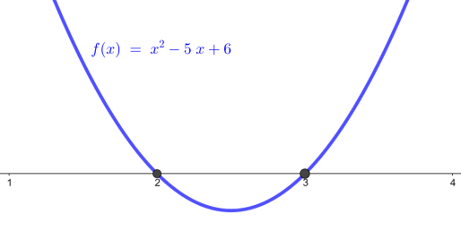
\includegraphics[width=\textwidth]{../Mathematik_1/Bilder/ungleichungen_quadratische_funktion_nullstellen.png}
\end{minipage}
\begin{minipage}{0.55\textwidth}
\begin{itemize}
\item Gezeigt ist der Graph der Funktion
\(
	f(x)=x^2-5x+6.
	\)
\item Positive Funktionswerte treten links der kleineren und rechts der gr��eren Nullstelle auf. Genau diese Bereiche bilden die zuvor berechnete L�sungsmenge.
\end{itemize}
\end{minipage}
\end{exabox}

\noindent\textbf{Bemerkungen:}
\begin{itemize}
\item Die L�sungsmenge l�sst sich damit sowohl rechnerisch als auch am Graphen erkennen.
\item Quadratische Terme lassen sich mithilfe ihrer Nullstellen faktorisieren:
\(
	ax^2+bx+c=a(x-x_1)(x-x_2).
	\)
\item Das Grundprinzip aus Nullstellenbestimmung und Vorzeichenanalyse bleibt auch bei polynomialen Ungleichungen h�herer Ordnung erhalten.
\end{itemize}

Bei einer \textbf{Bruchungleichung} kommt eine weitere Schwierigkeit hinzu: Das Vorzeichen eines Bruches h�ngt sowohl vom Z�hler als auch vom Nenner ab. Gleichzeitig darf der Nenner niemals Null werden. Eine Multiplikation mit dem Nenner ist deshalb erst dann m�glich, wenn bekannt ist, welches Vorzeichen dieser besitzt.

Besonders einfach ist der Fall, dass der Bruch mit Null verglichen wird. Ein Bruch ist nichtnegativ, wenn Z�hler und Nenner dasselbe Vorzeichen besitzen oder der Z�hler Null ist.

\begin{exabox}{L�sen einer Bruchungleichung mit rechter Seite Null}{ }
Betrachtet wird

$$
\frac{2x-1}{x+4}\geq0.
$$

Der Nenner darf nicht verschwinden, also gilt zun�chst

$$
x\neq-4.
$$

Damit der Bruch nichtnegativ ist, m�ssen Z�hler und Nenner gleiches Vorzeichen besitzen:

$$
\begin{array}{rcl}
\dfrac{2x-1}{x+4}\geq0
&\Leftrightarrow&
\begin{cases}
2x-1\geq0 \land x+4>0,\\
2x-1\leq0 \land x+4<0
\end{cases}
\\[2ex]
&\Leftrightarrow&
\begin{cases}
x\geq\dfrac12 \land x>-4,\\
x\leq\dfrac12 \land x<-4
\end{cases}
\\[2ex]
&\Leftrightarrow&
\begin{cases}
x\geq\dfrac12,\\
x<-4.
\end{cases}
\end{array}
$$

Die beiden F�lle werden vereinigt. Damit ergibt sich

$$
x\in(-\infty,-4)\cup\left[\frac12,\infty\right).
$$

\end{exabox}

Steht auf der rechten Seite dagegen eine von Null verschiedene Zahl, kann nicht allein das Vorzeichen des gesamten Bruches betrachtet werden. Um den Nenner zu beseitigen, m�sste mit \(x+4\) multipliziert werden. Dabei h�ngt die Richtung des Ungleichheitszeichens davon ab, ob \(x+4\) positiv oder negativ ist. Deshalb wird \textbf{zuerst das Vorzeichen des Nenners unterschieden}.

\begin{exabox}{L�sen einer Bruchungleichung mit konstanter rechter Seite}{ }
Betrachtet wird

$$
\frac{2x-1}{x+4}\geq3.
$$

Der Nenner verschwindet f�r \(x=-4\). Dieser Wert geh�rt nicht zum Definitionsbereich. F�r alle �brigen Werte werden zwei F�lle unterschieden.

$$
\begin{array}{rcll}
\dfrac{2x-1}{x+4}\geq3
&\Leftrightarrow&
\begin{cases}
x+4>0 \land 2x-1\geq3(x+4),\\
x+4<0 \land 2x-1\leq3(x+4)
\end{cases}
& \text{Nenner-Vorzeichen}
\\[3ex]
&\Leftrightarrow&
\begin{cases}
x>-4 \land x\leq-13,\\
x<-4 \land x\geq-13
\end{cases}
& \text{Ungleichungen l�sen}
\\[3ex]
&\Leftrightarrow&
\begin{cases}
x\in\emptyset,\\
x\in[-13,-4)
\end{cases}
& \text{F�lle auswerten}
\\[3ex]
&\Leftrightarrow&
x\in[-13,-4).
& \text{vereinigen}
\end{array}
$$

Im ersten Fall widersprechen sich die Bedingungen \(x>-4\) und \(x\leq-13\); dieser Fall liefert daher keine L�sung. Im zweiten Fall m�ssen \(x<-4\) und \(x\geq-13\) gleichzeitig erf�llt sein. Daraus entsteht das Intervall \([-13,-4)\).
\end{exabox}

Bei einer \textbf{Betragsungleichung} entsteht die Fallunterscheidung aus der Definition des Betrags. Der Betrag eines Ausdrucks h�ngt davon ab, ob dieser Ausdruck nichtnegativ oder negativ ist:

$$
|T|=
\begin{cases}
T,&T\geq0,\\
-T,&T<0.
\end{cases}
$$

F�r die Ungleichung \(|x-7|<5\) wird deshalb das Vorzeichen von \(x-7\) unterschieden.

\begin{exabox}{L�sen einer Betragsungleichung}{ }

$$
\begin{array}{rcl}
|x-7|<5
&\Leftrightarrow&
\begin{cases}
x-7\geq0 \land x-7<5,\\
x-7<0 \land -(x-7)<5
\end{cases}
\\[2ex]
&\Leftrightarrow&
\begin{cases}
x\geq7 \land x<12,\\
x<7 \land x>2
\end{cases}
\\[2ex]
&\Leftrightarrow&
\begin{cases}
x\in[7,12),\\
x\in(2,7)
\end{cases}
\\[2ex]
&\Leftrightarrow&
x\in(2,12).
\end{array}
$$

\end{exabox}

Bei einfachen Betragsungleichungen l�sst sich dasselbe Ergebnis auch unmittelbar aus der Bedeutung des Betrags ablesen:

$$
|x-7|<5
\;\Leftrightarrow\;
-5<x-7<5
\;\Leftrightarrow\;
2<x<12.
$$

Die ausf�hrliche Fallunterscheidung bleibt dennoch wichtig, da sie auch dann funktioniert, wenn kompliziertere Ausdr�cke innerhalb des Betrags auftreten.

Treten mehrere dieser Strukturen gleichzeitig auf, m�ssen die notwendigen Fallunterscheidungen miteinander kombiniert werden. Bei einem Betrag im Z�hler und einem variablen Nenner muss beispielsweise sowohl das Vorzeichen des Nenners als auch das Vorzeichen des Ausdrucks innerhalb des Betrags ber�cksichtigt werden.
 

\end{document}
